\chapter{Prezentarea aplica\c tiei}

Aplica\c tia ManFast ruleaz\u a \^in browser la \texttt{http://localhost:5173} (frontend) \c si comunic\u a cu API-ul Express la portul 5000. \^In acest capitol sunt ilustrate interfe\c tele principale.

\section{Utilizarea aplica\c tiei — perspectiva \linebreak utilizatorului}

\subsection{Pagina principal\u a}

Pagina principal\u a afi\c seaz\u a evenimentele viitoare sub form\u a de list\u a orizontal\u a. Componenta \texttt{EventSearchFilters} permite filtrarea dup\u a nume, jude\c t (select din 42 jude\c te) \c si dat\u a. Evenimentele expirate (data + durata) nu apar \^in list\u a.

Utilizatorul neautentificat poate naviga \c si filtra evenimente. Pentru cump\u arare bilet este necesar\u a autentificarea. Designul folose\c ste carduri \texttt{EventListItem} cu titlu, loca\c tie, pre\c t \c si locuri disponibile. Navbar-ul con\c tine link-uri c\u atre ,,Evenimente``, ,,Biletele mele`` \c si ,,Profil`` (vizibile doar autentificat), plus buton ,,Panou Admin`` pentru rol admin.

Filtrarea pe jude\c t utilizeaz\u a lista complet\u a jude\c telor din \texttt{constants/judete.js}, aliniat\u a la organizarea administrativ\u a din Rom\^ania. Filtrul pe dat\u a permite restr\^angerea rezultatelor la o zi specific\u a, util \^in planificarea particip\u arii la competi\c tii.

\begin{figure}[htbp]
	\centering
	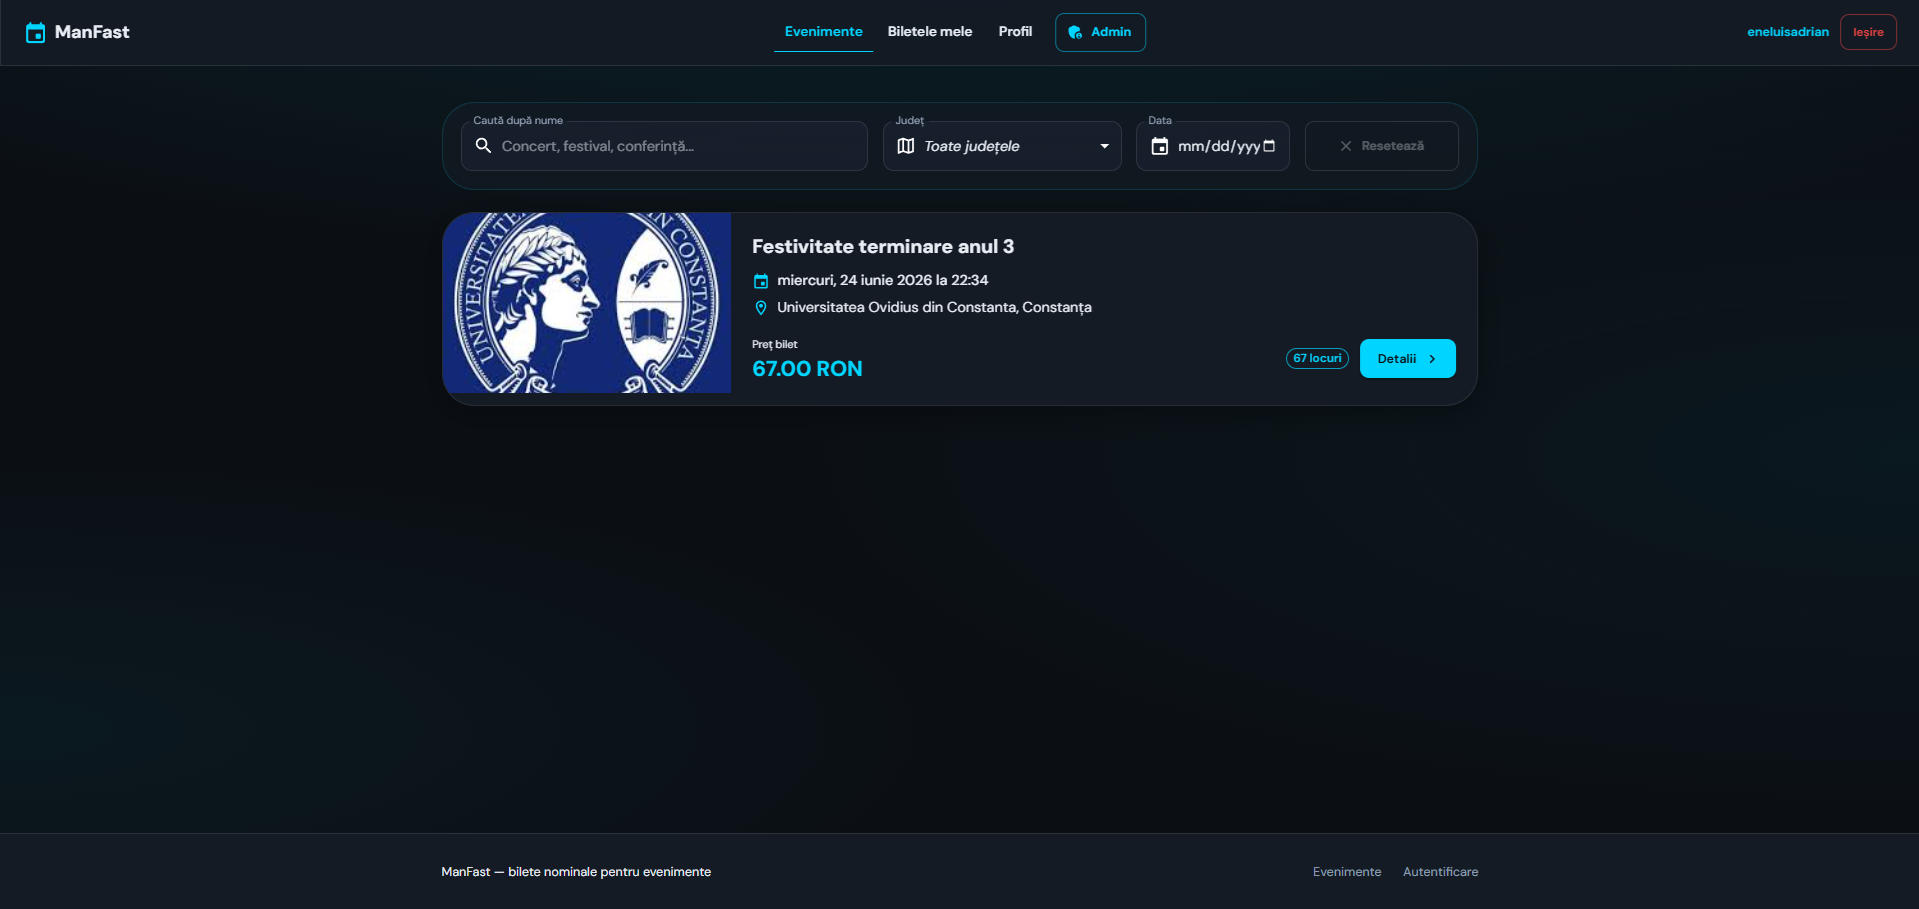
\includegraphics[width=1\textwidth]{paginaprincipala.png}
	\caption{Pagina principal\u a — list\u a evenimente \c si filtre}
	\label{fig:l2f1}
\end{figure}



\subsection{Detalii eveniment}

Pagina \texttt{/events/:id} prezint\u a titlul, galeria de imagini, descrierea, data, jude\c tul, localitatea, loca\c tia, pre\c tul \c si locurile disponibile. Utilizatorul autentificat poate ad\u auga unul sau mai multe c\^ampuri ,,Nume participant`` \c si ini\c tia plata Stripe.

Galeria de imagini suport\u a mai multe fi\c siere \^inc\u arcate de admin (max 8, 5MB/fi\c sier). Layout-ul este responsive: pe desktop, detaliile \c si formularul de cump\u arare pot ap\u area \^in coloane; pe mobil, stiv\u a vertical\u a. Validarea frontend verific\u a c\u a toate numele sunt completate \^inainte de apelul API. La succes, utilizatorul este redirectat c\u atre Stripe Checkout hosted page — datele cardului nu tranziteaz\u a serverul ManFast.



\begin{figure}[htbp]
	\centering
	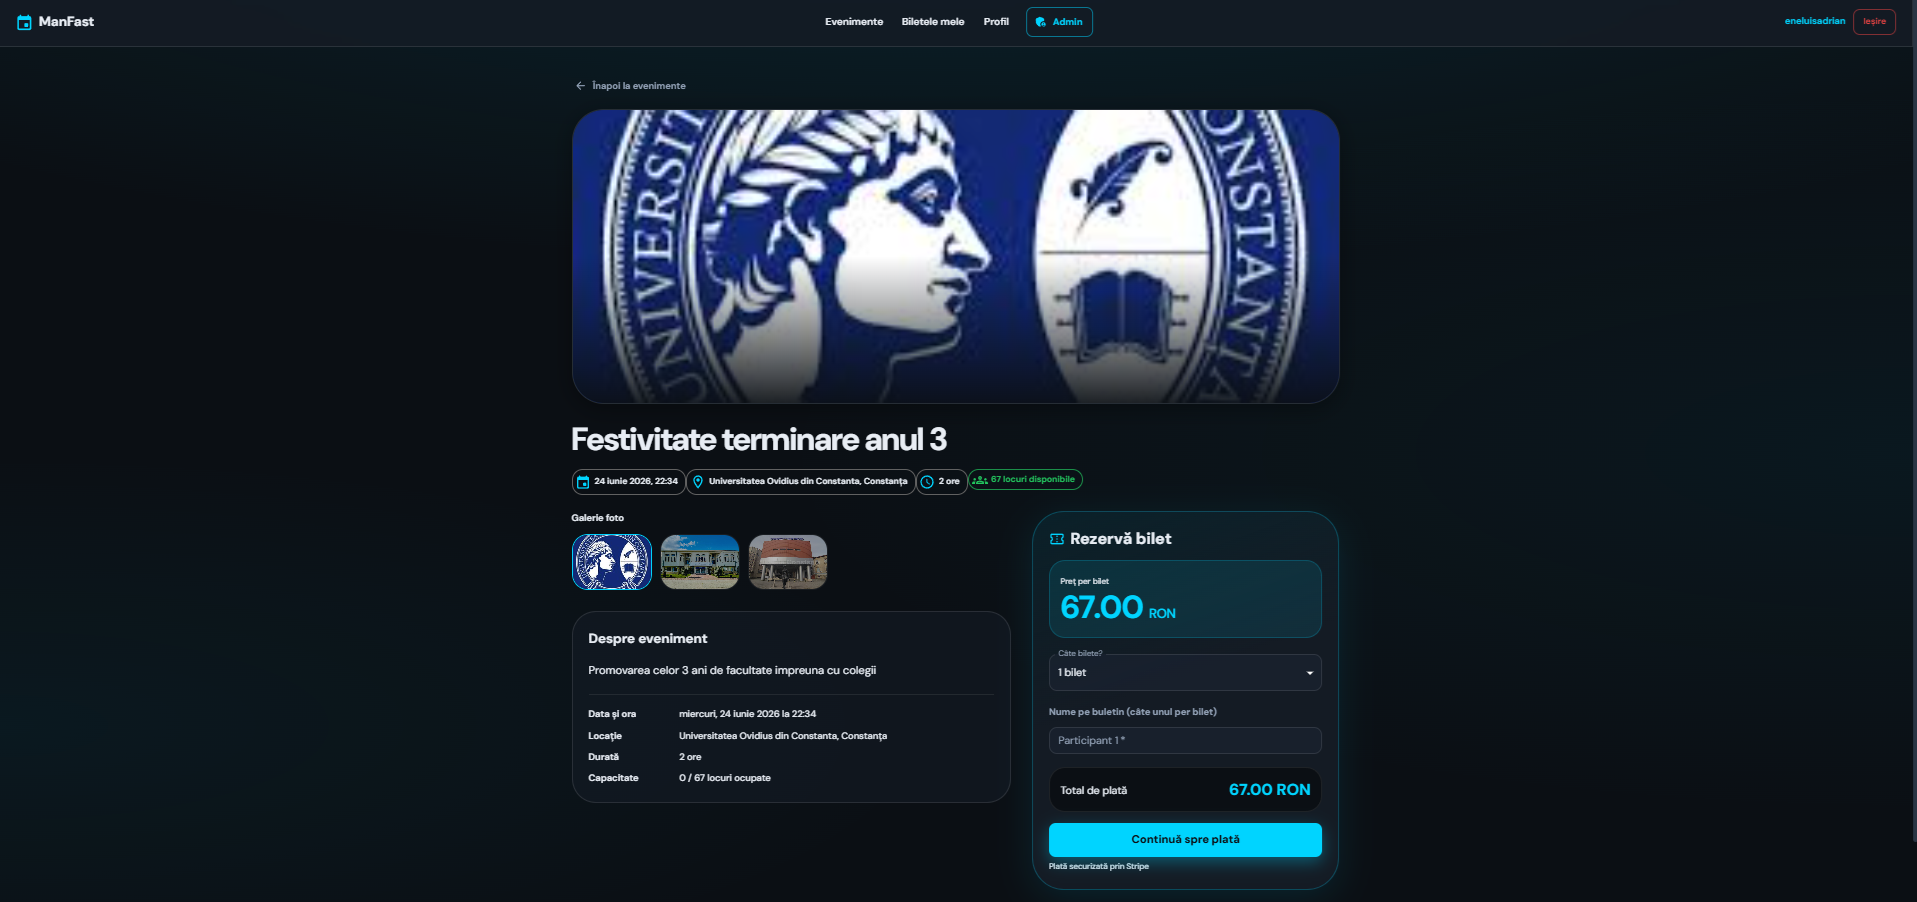
\includegraphics[width=1\textwidth]{Pagina_detalii_eveniment_si_formular_bilete.png}
	\caption{Pagina detalii eveniment \c si formular bilete}
	\label{fig:l2f1}
\end{figure}

\subsection{\^Inregistrare cont — pasul 1}

Formularul de \^inregistrare colecteaz\u a username, email, telefon, parol\u a. La submit se apeleaz\u a \texttt{POST /api/auth/register} \c si se trece la ecranul de verificare.

\begin{figure}[htbp]
	\centering
	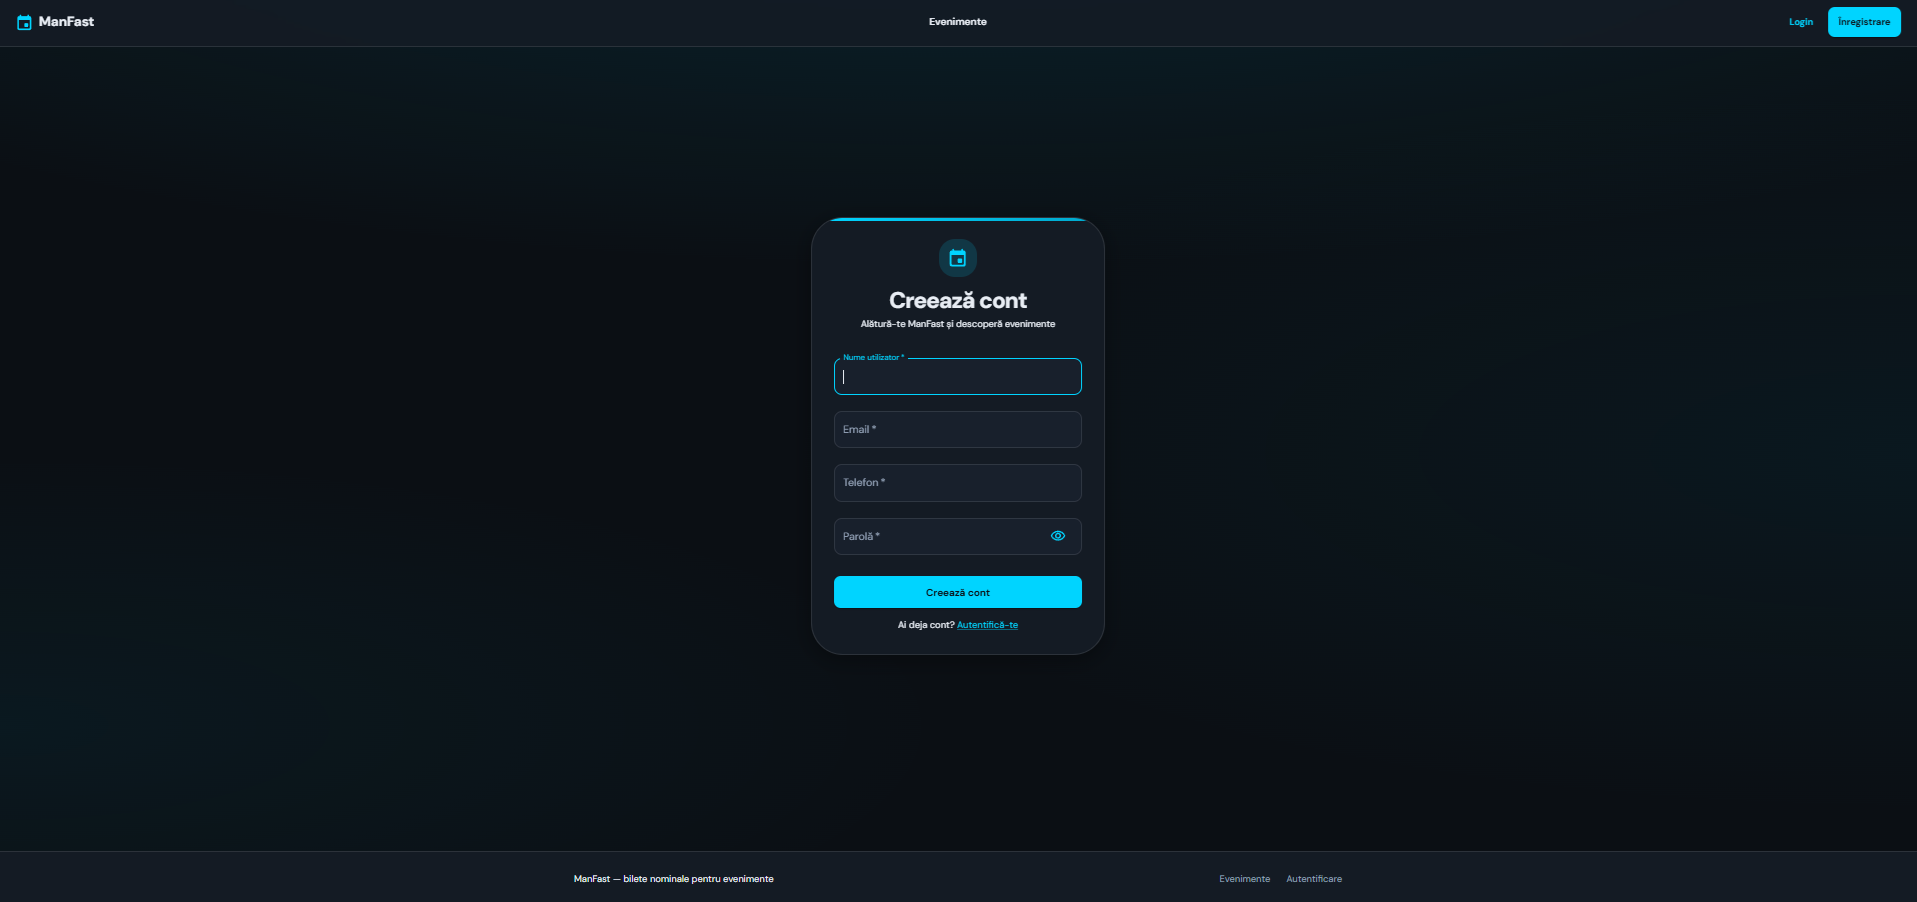
\includegraphics[width=1\textwidth]{Formular_inregistrare.png}
	\caption{Formular \^inregistrare}
	\label{fig:l2f1}
\end{figure}

\subsection{Verificare email — pasul 2}

Utilizatorul introduce codul de 6 cifre primit pe email. Op\c tiuni: retrimite cod, \^inapoi la formular.

\begin{figure}[htbp]
	\centering
	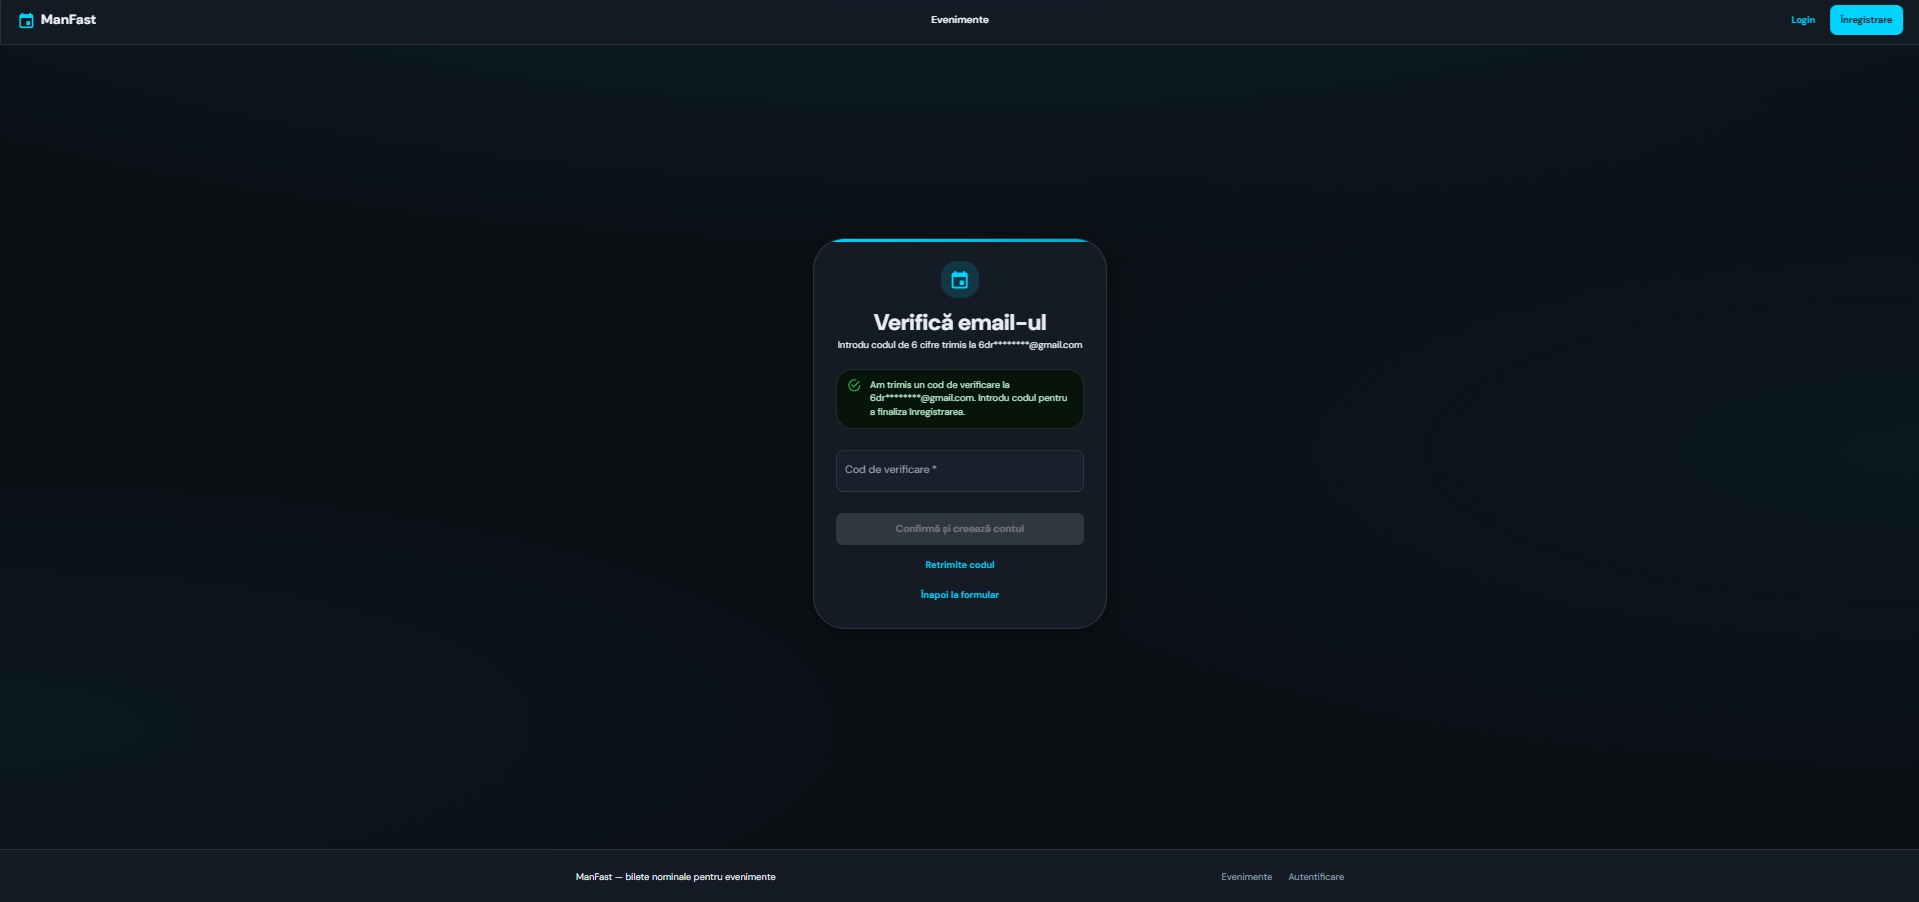
\includegraphics[width=1\textwidth]{Verificare email cu_cod.png}
	\caption{Verificare email cu cod}
	\label{fig:l2f1}
\end{figure}

\subsection{Autentificare}

Pagina \texttt{/login} permite autentificarea. Link-uri c\u atre ,,Am uitat parola`` \c si ,,\^Inregistreaz\u a-te`` (transfer email/parol\u a prin state).

\begin{figure}[htbp]
	\centering
	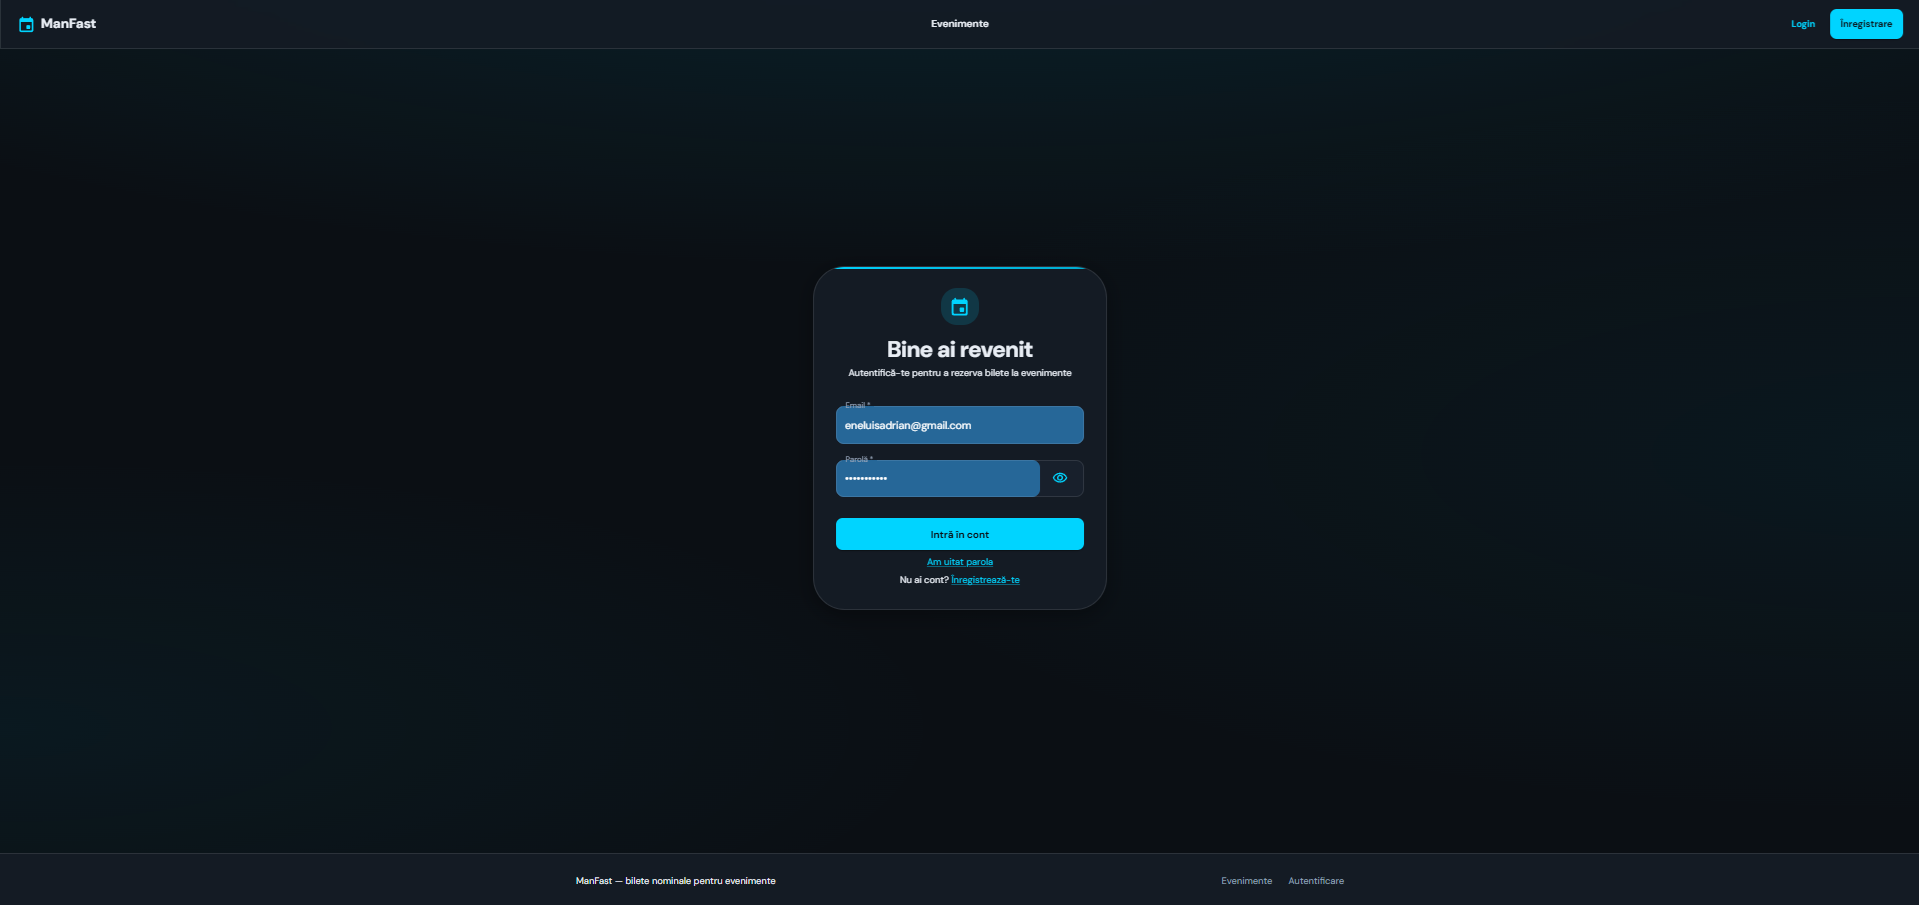
\includegraphics[width=1\textwidth]{Pagina login.png}
	\caption{Pagina login}
	\label{fig:l2f1}
\end{figure}

\subsection{Confirmare plat\u a}

Dup\u a Stripe Checkout, utilizatorul revine la \texttt{/payment-success?session\_id=...}. Frontend confirm\u a plata \c si redirec\c tioneaz\u a spre bilete.

\begin{figure}[htbp]
	\centering
	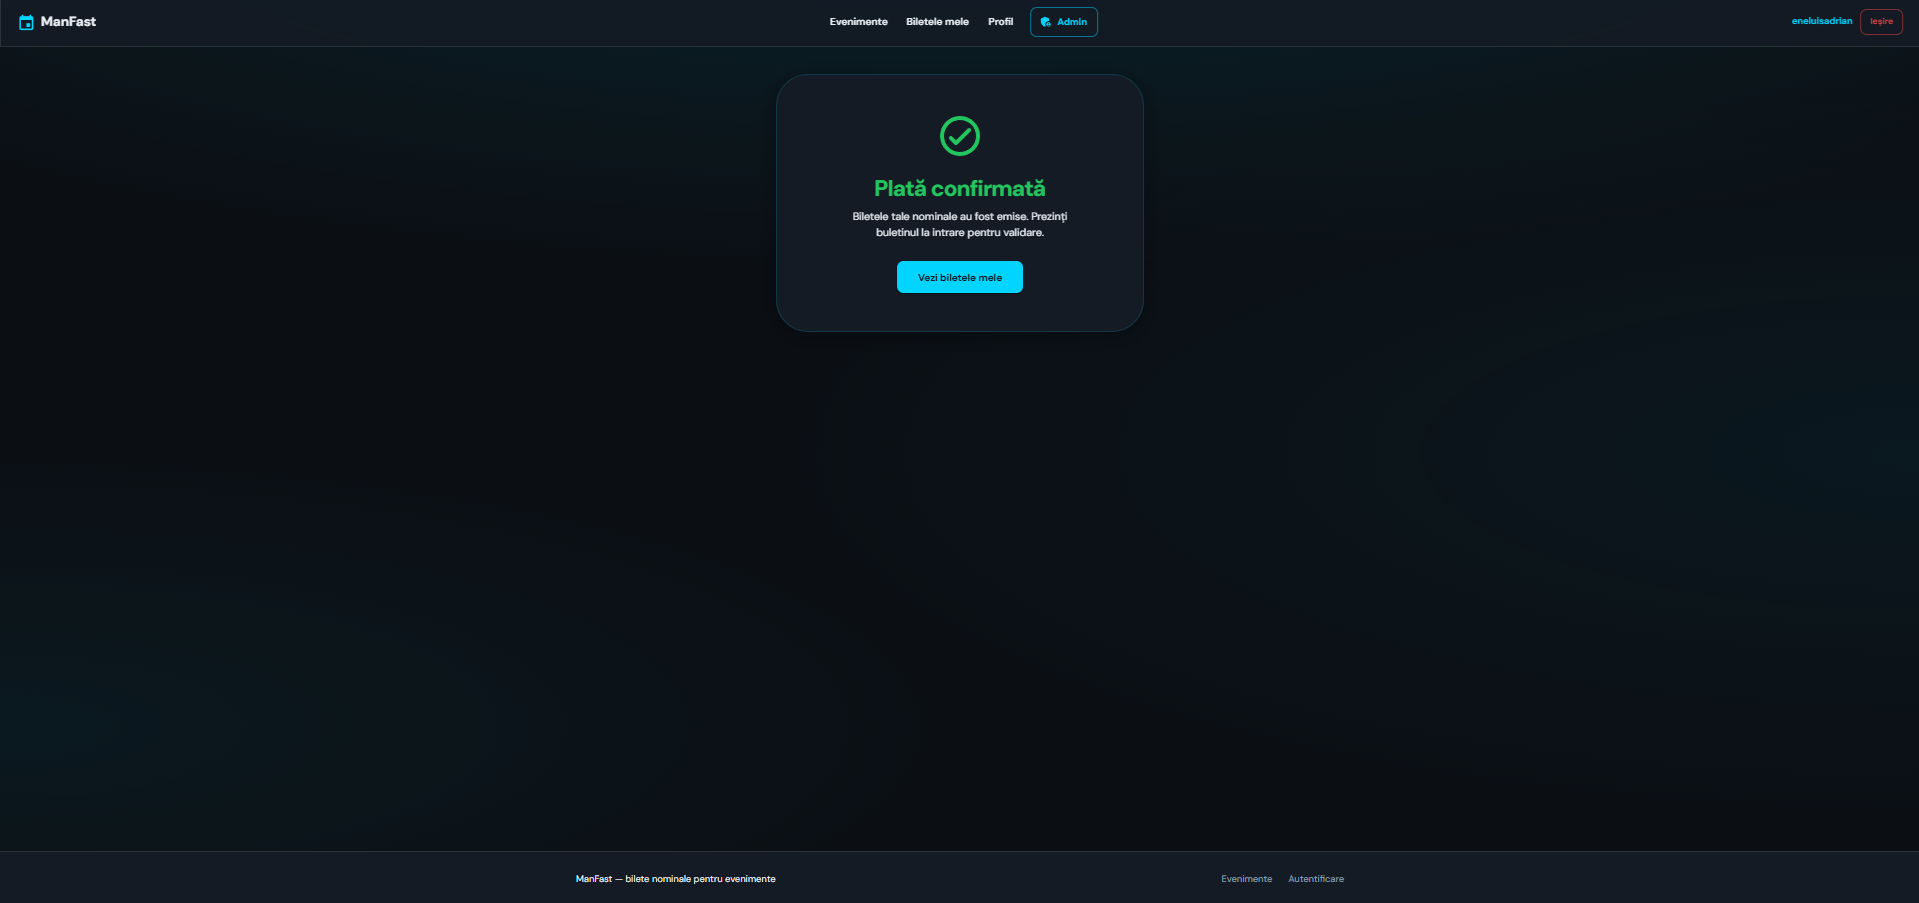
\includegraphics[width=1\textwidth]{Pagina succes plat ˘ a.png}
	\caption{Pagina succes plat\u a}
	\label{fig:l2f1}
\end{figure}

\subsection{Biletele mele}

\texttt{/my-tickets} grupeaz\u a biletele \^in ,,viitoare`` \c si ,,trecute``. Fiecare card arat\u a evenimentul, numele de pe bilet, status (Pl\u atit / Check-in / Expirat).

\begin{figure}[htbp]
	\centering
	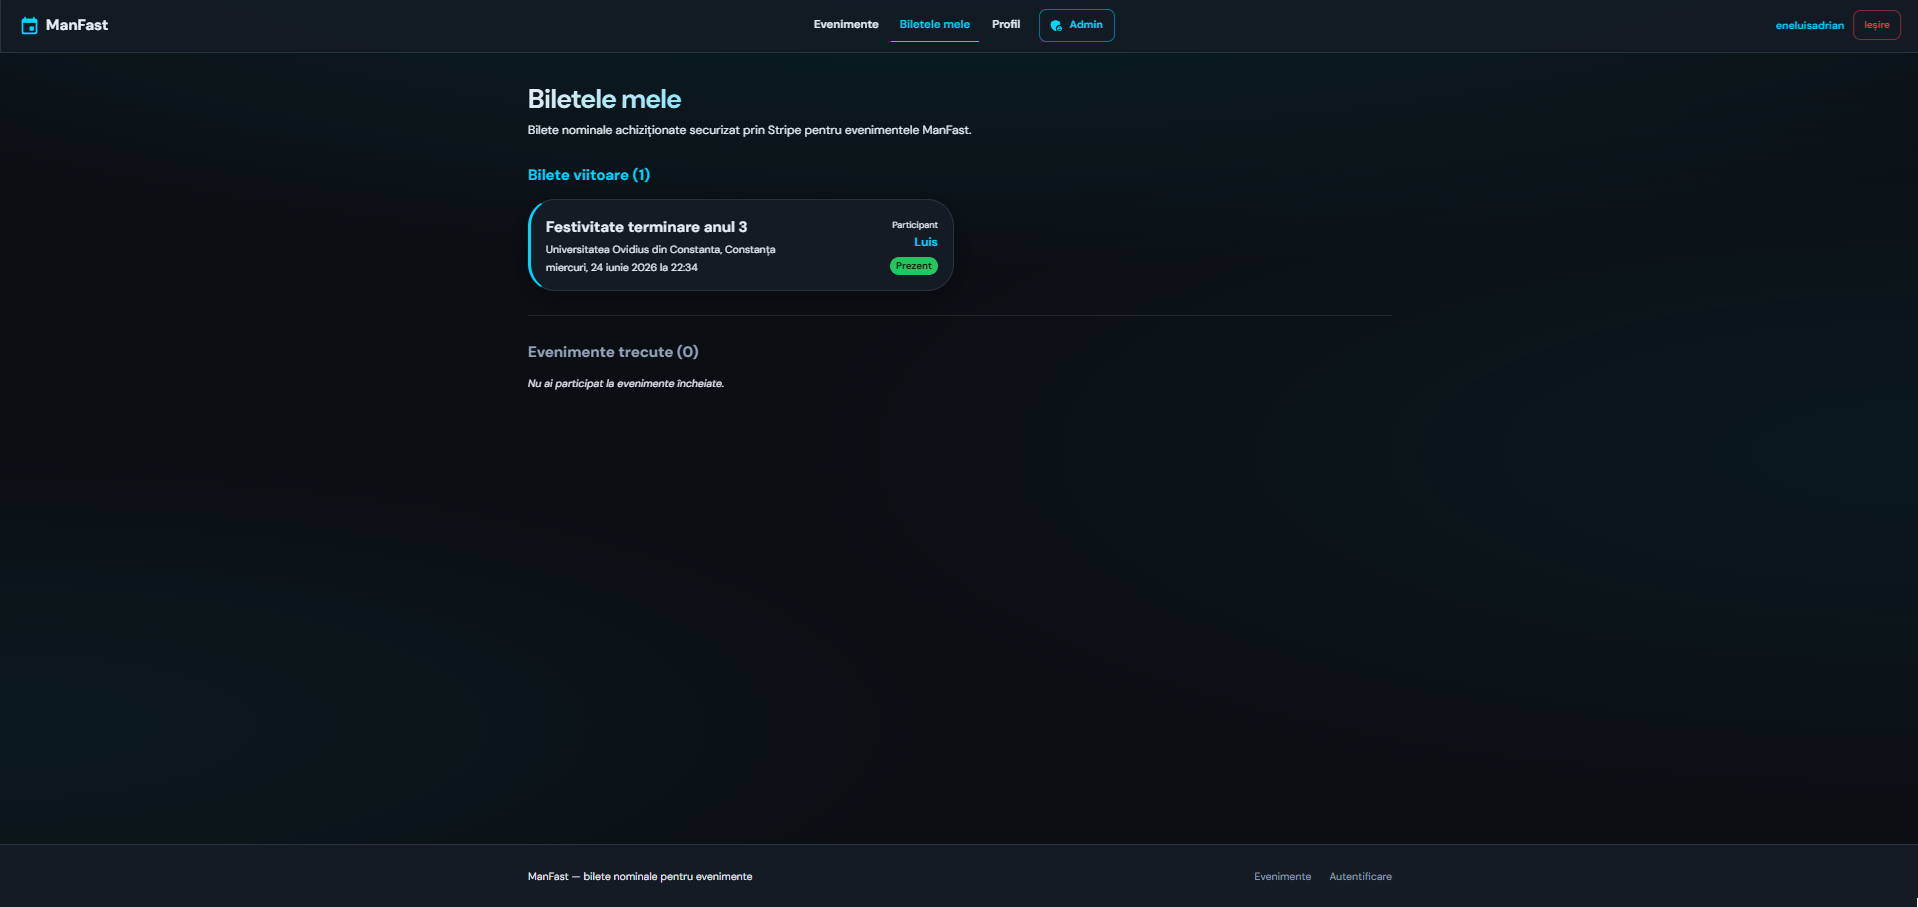
\includegraphics[width=1\textwidth]{Biletele mele.png}
	\caption{Biletele mele}
	\label{fig:l2f1}
\end{figure}

\subsection{Profil utilizator}

\texttt{/profile}: mod vizualizare \c si mod editare; schimbare parol\u a; zon\u a ro\c sie \c stergere cont.

\begin{figure}[htbp]
	\centering
	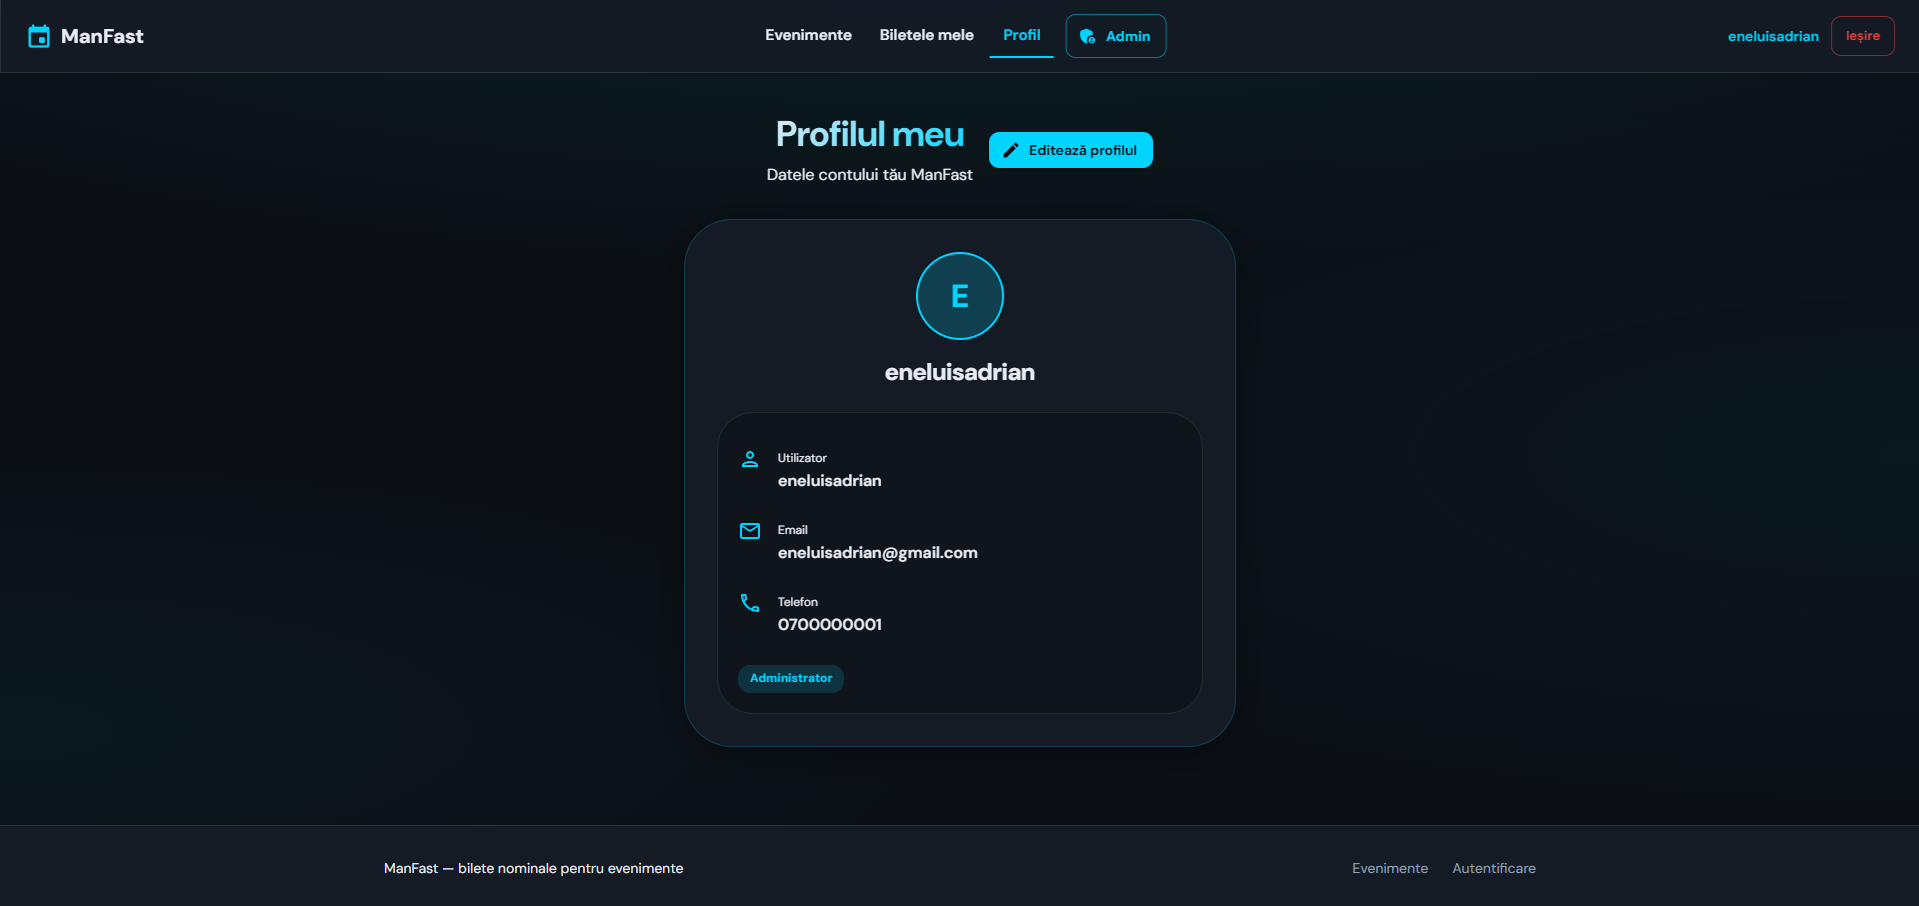
\includegraphics[width=1\textwidth]{Profil utilizator.png}
	\caption{Profil utilizator}
	\label{fig:l2f1}
\end{figure}

\subsection{Resetare parol\u a — pasul 1 (op\c tional)}

Formularul ,,Am uitat parola`` accept\u a email sau telefon; backend-ul trimite link de reset pe email (mesaj generic pentru confiden\c tialitate).

\begin{figure}[htbp]
	\centering
	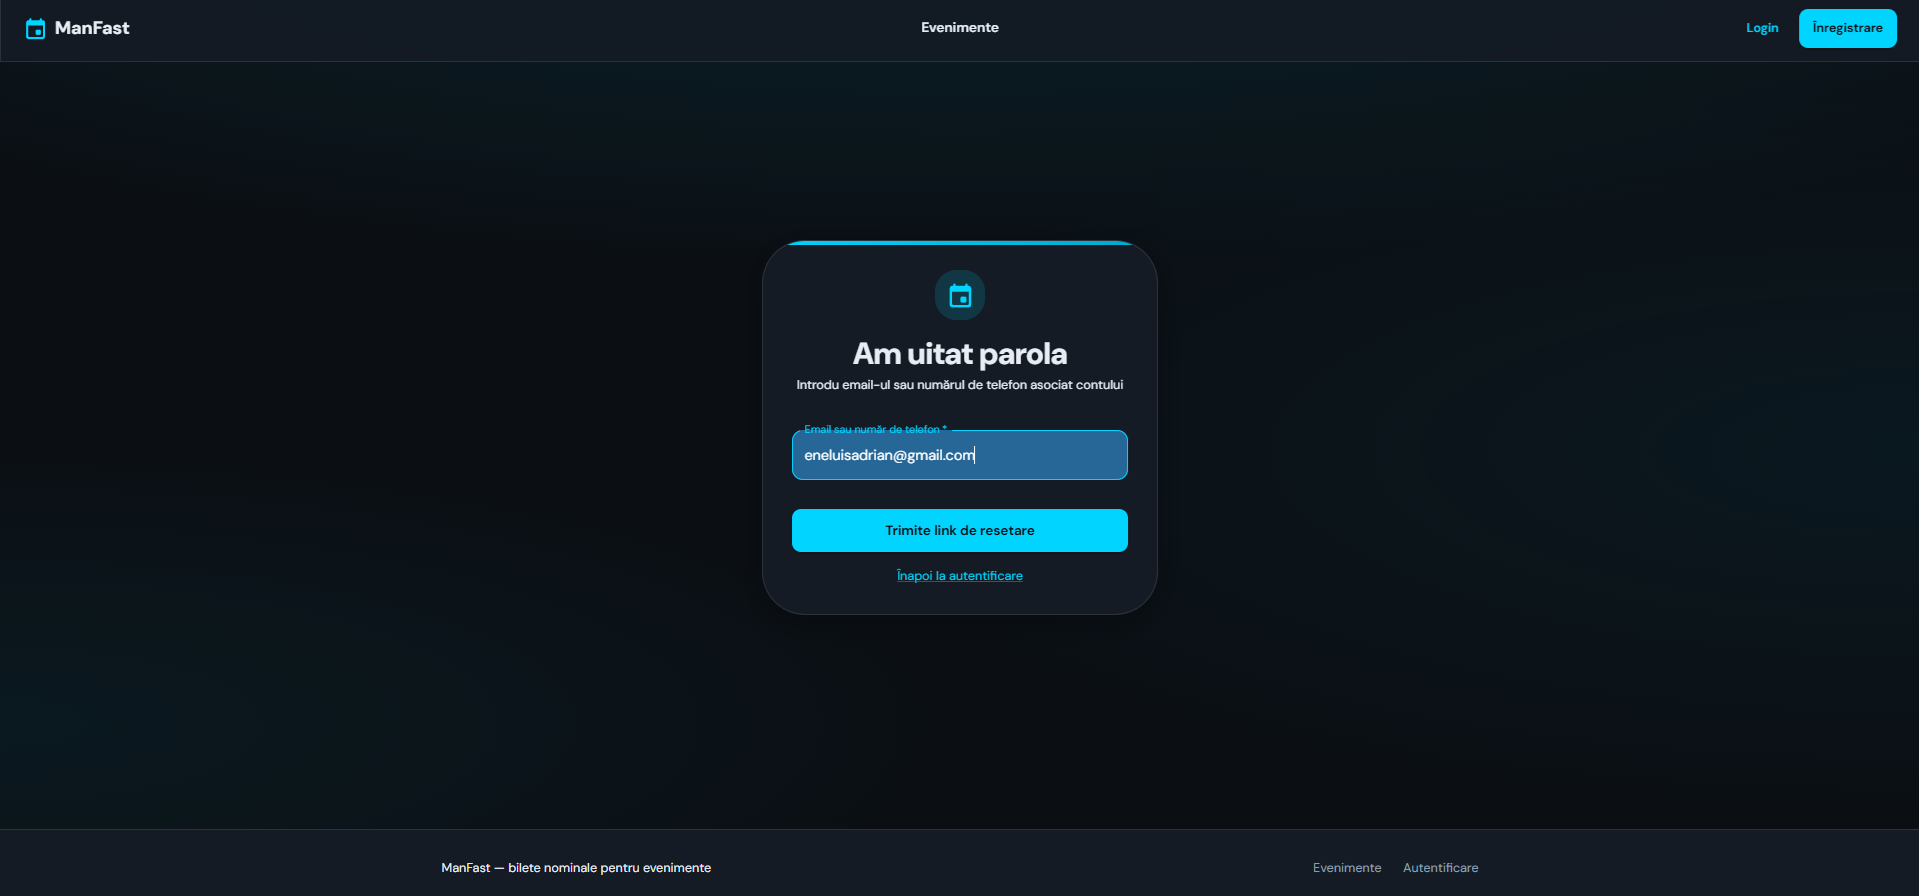
\includegraphics[width=1\textwidth]{Pagina Am uitat parola (opt¸ional).png}
	\caption{Pagina Am uitat parola (op\c tional)}
	\label{fig:l2f1}
\end{figure}

\subsection{Resetare parol\u a — pasul 2 (op\c tional)}

Dup\u a solicitarea reset\u arii, utilizatorul acceseaz\u a link-ul din email (\texttt{/reset-password-\linebreak token=...}) \c si seteaz\u a parola nou\u a. Token-ul este validat server-side (hash SHA-256, expirare 1h).

\begin{figure}[htbp]
	\centering
	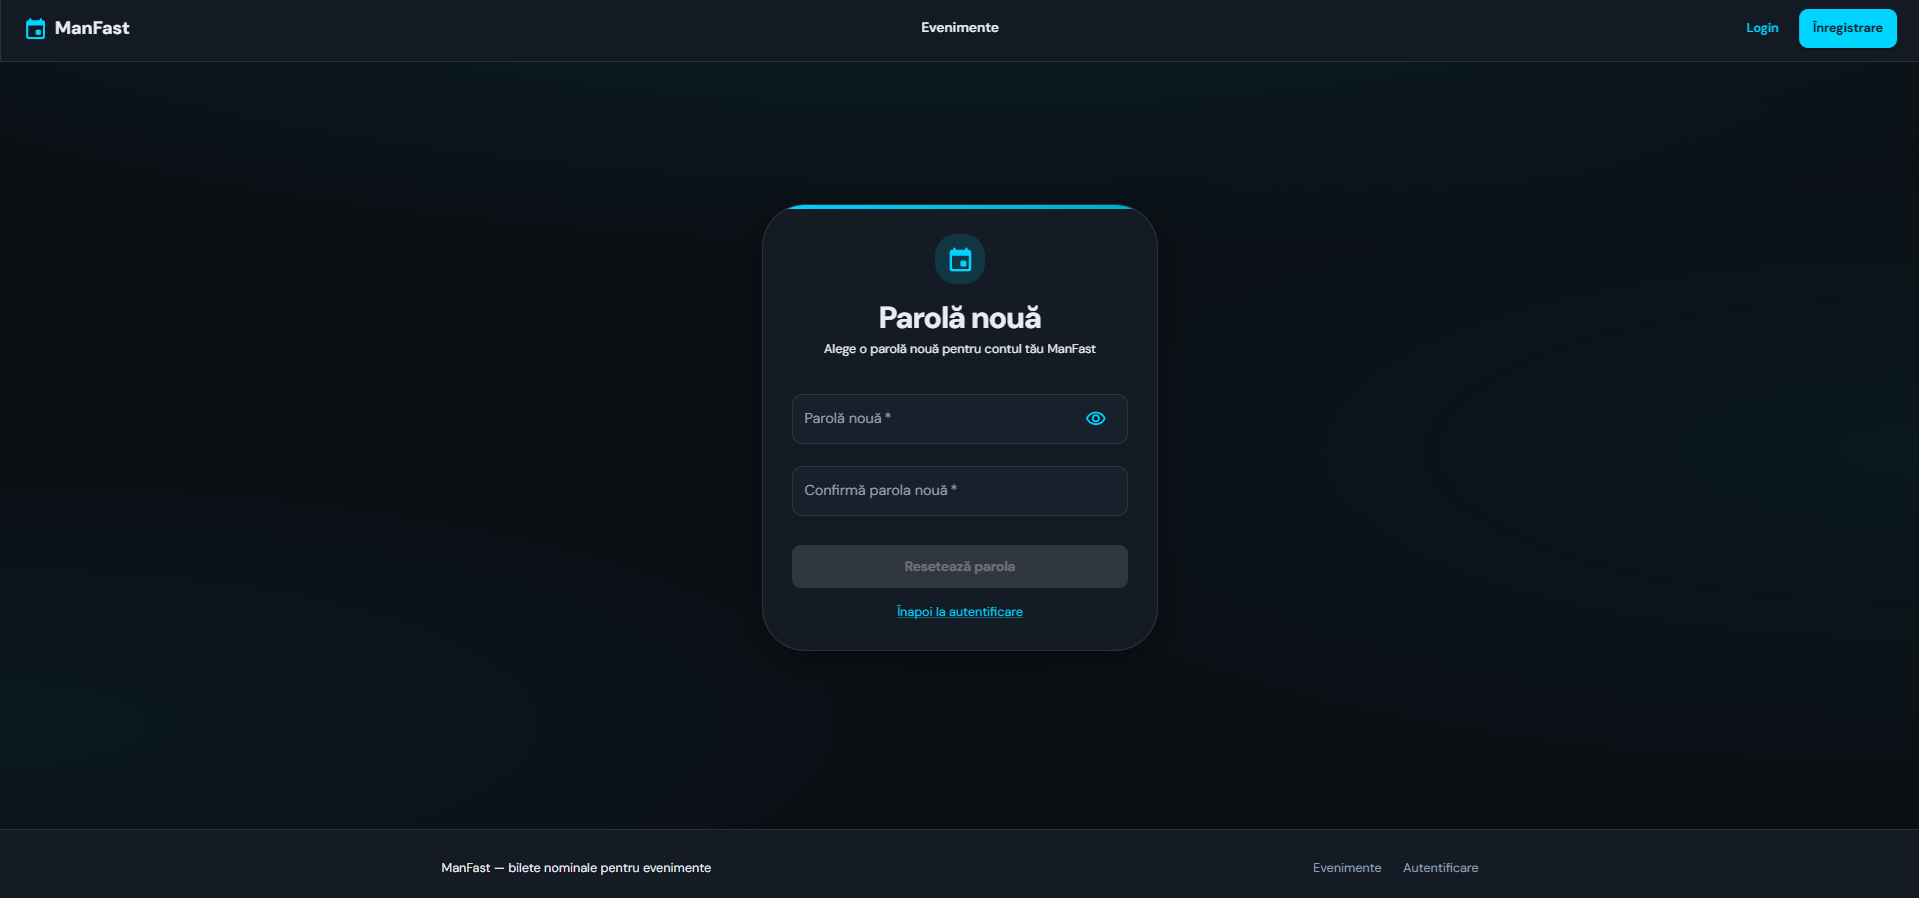
\includegraphics[width=1\textwidth]{Formular parola nou ˘ a (reset).png}
	\caption{Formular parola nou\u a (reset)}
	\label{fig:l2f1}
\end{figure}


\section{Experien\c ta utilizatorului \c si design responsive}

\subsection{Parcursul utilizatorului (user journey)}

Fluxul complet al unui participant nou poate fi rezumat astfel: descoperire eveniment pe Home $\rightarrow$ consultare detalii $\rightarrow$ redirect la Login/Register dac\u a nu este autentificat $\rightarrow$ \linebreak \^inregistrare cu verificare email $\rightarrow$ revenire la eveniment $\rightarrow$ completare nume participan\c ti $\rightarrow$ plat\u a Stripe $\rightarrow$ confirmare $\rightarrow$ vizualizare bilet \^in Biletele mele $\rightarrow$ prezentare la check-in (validat de admin)

Fiecare pas este marcat de feedback vizual: st\u ari de \^inc\u arcare (\texttt{CircularProgress}), mesaje de eroare contextualizate, redirect automat dup\u a ac\c tiuni reu\c site. Transferul email/\linebreak parol\u a de la Login la Register (via \texttt{location.state}) reduce fric\c tiunea pentru utilizatorii care \^incep de pe pagina gre\c sit\u a.

\subsection{Adaptare mobil \c si accesibilitate}

Material UI 9 ofer\u a componente responsive (\texttt{Grid}, \texttt{Stack}, \texttt{useMediaQuery}). Navbar-ul comut\u a la meniul hamburger pe ecrane \^inguste; filtrele pe Home se stiveaz\u a vertical. Formularele de autentificare sunt centrate \^in \texttt{AuthCard} cu l\u a\c time maxim\u a, u\c sor de utilizat pe telefon.

Au fost remediate probleme de accesibilitate: focus corect dup\u a \^inchiderea meniului mobil (evitare \texttt{aria-hidden} pe elemente focusabile), utilizarea etichetelor \texttt{label} pe c\^ampuri, contrast ridicat \^in tema dark (cyan pe fundal \^intunecat).

\subsection{Mesaje de eroare \c si st\u ari goale}

Listele goale (f\u ar\u a evenimente, f\u ar\u a bilete) afi\c seaz\u a text explicativ \c si sugestii (ex. ,,Modific\u a filtrele`` sau ,,Cump\u ar\u a primul bilet``). Erorile API (429 rate limit, 401 sesiune expirat\u a) sunt traduse \^in mesaje inteligibile, f\u ar\u a detalii tehnice expuse utilizatorului final.

\section{Utilizarea aplica\c tiei — perspectiva administratorului}

Administratorul acceseaz\u a \texttt{/admin} dup\u a autentificare cu rol \texttt{admin}. Componenta \linebreak \texttt{AdminRoute} verific\u a token JWT \c si rol; utilizatorii obi\c snui\c ti sunt redirec\c tiona\c ti.

Panoul centralizeaz\u a gestionarea evenimentelor \c si a participan\c tilor. Administratorul poate crea evenimente noi, edita pe cele existente (inclusiv ad\u augare imagini incremental), \c sterge evenimente (cu confirmare dialog) \c si vizualiza participan\c ti cu status check-in. Gestionarea administratorilor se face \^intr-un dialog separat, protejat de parol\u a de autorizare configurat\u a \^in \texttt{.env}.

\subsection{Panou admin — dashboard}

List\u a evenimente cu ac\c tiuni editare/\c stergere; tab participan\c ti; check-in.

\begin{figure}[htbp]
	\centering
	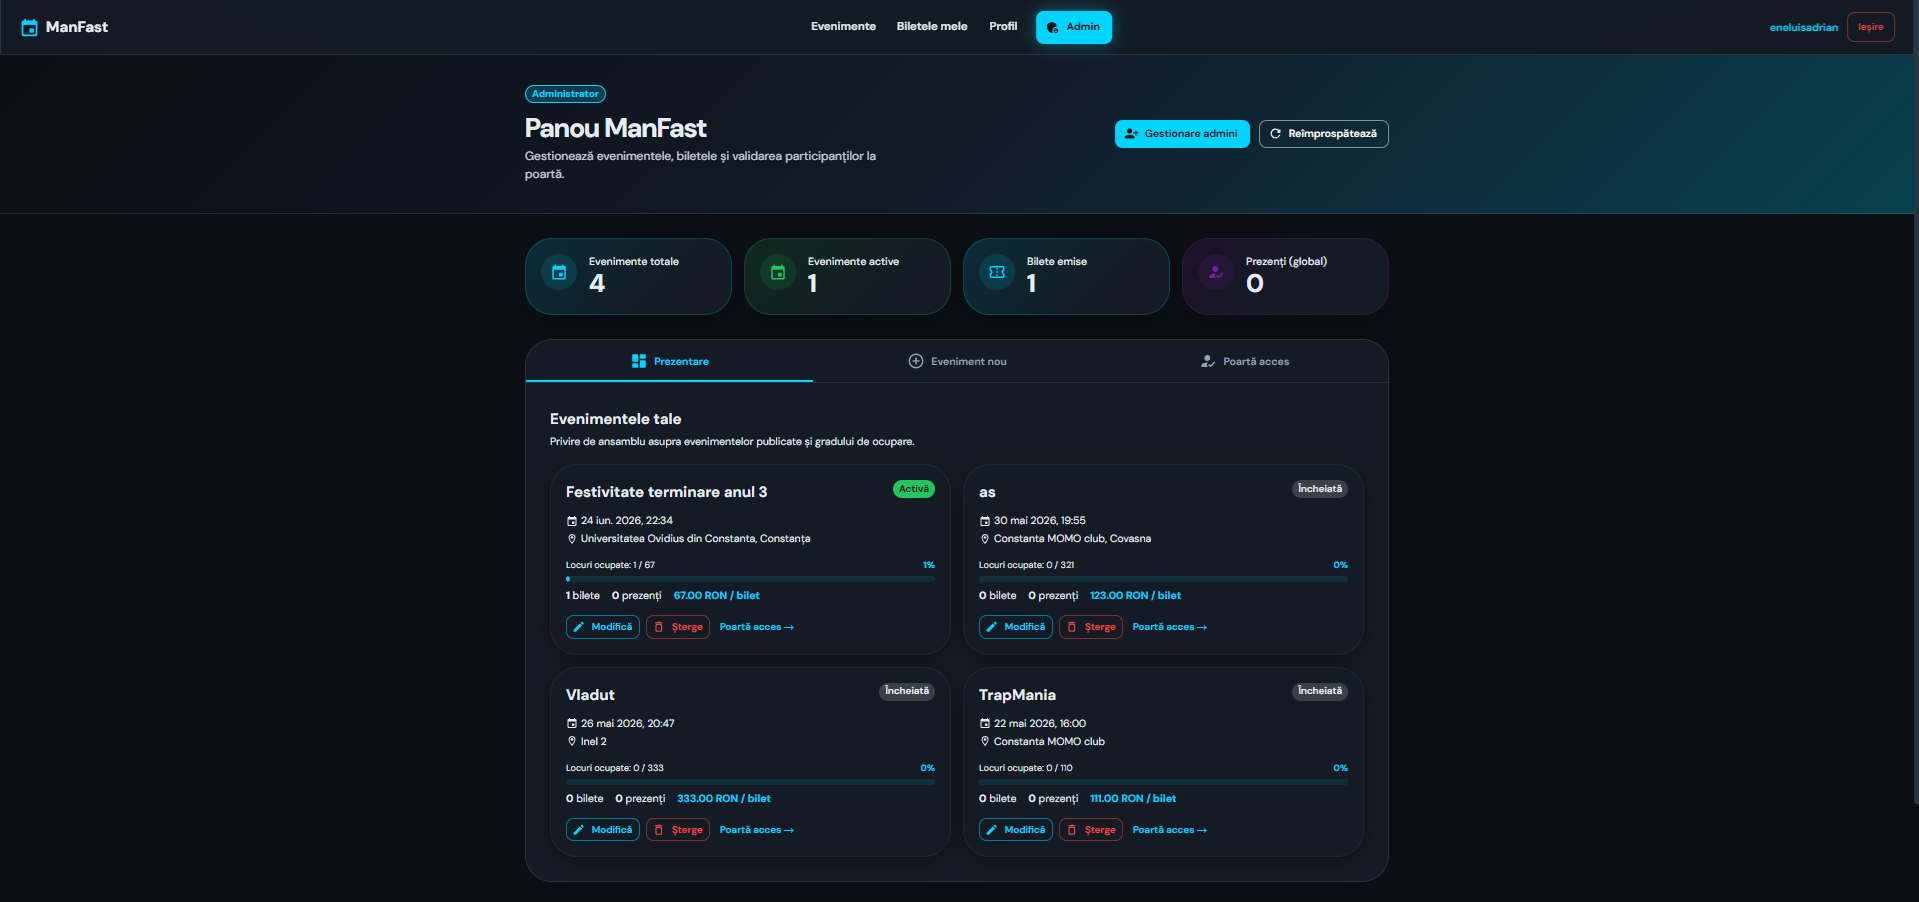
\includegraphics[width=1\textwidth]{Panou admin — dashboard.png}
	\caption{Panou admin — dashboard}
	\label{fig:l2f1}
\end{figure}

\subsection{Creare / editare eveniment}

Dialog cu c\^ampuri: titlu, descriere, dat\u a, jude\c t, localitate, pre\c t, locuri, durat\u a, upload imagini.

\begin{figure}[htbp]
	\centering
	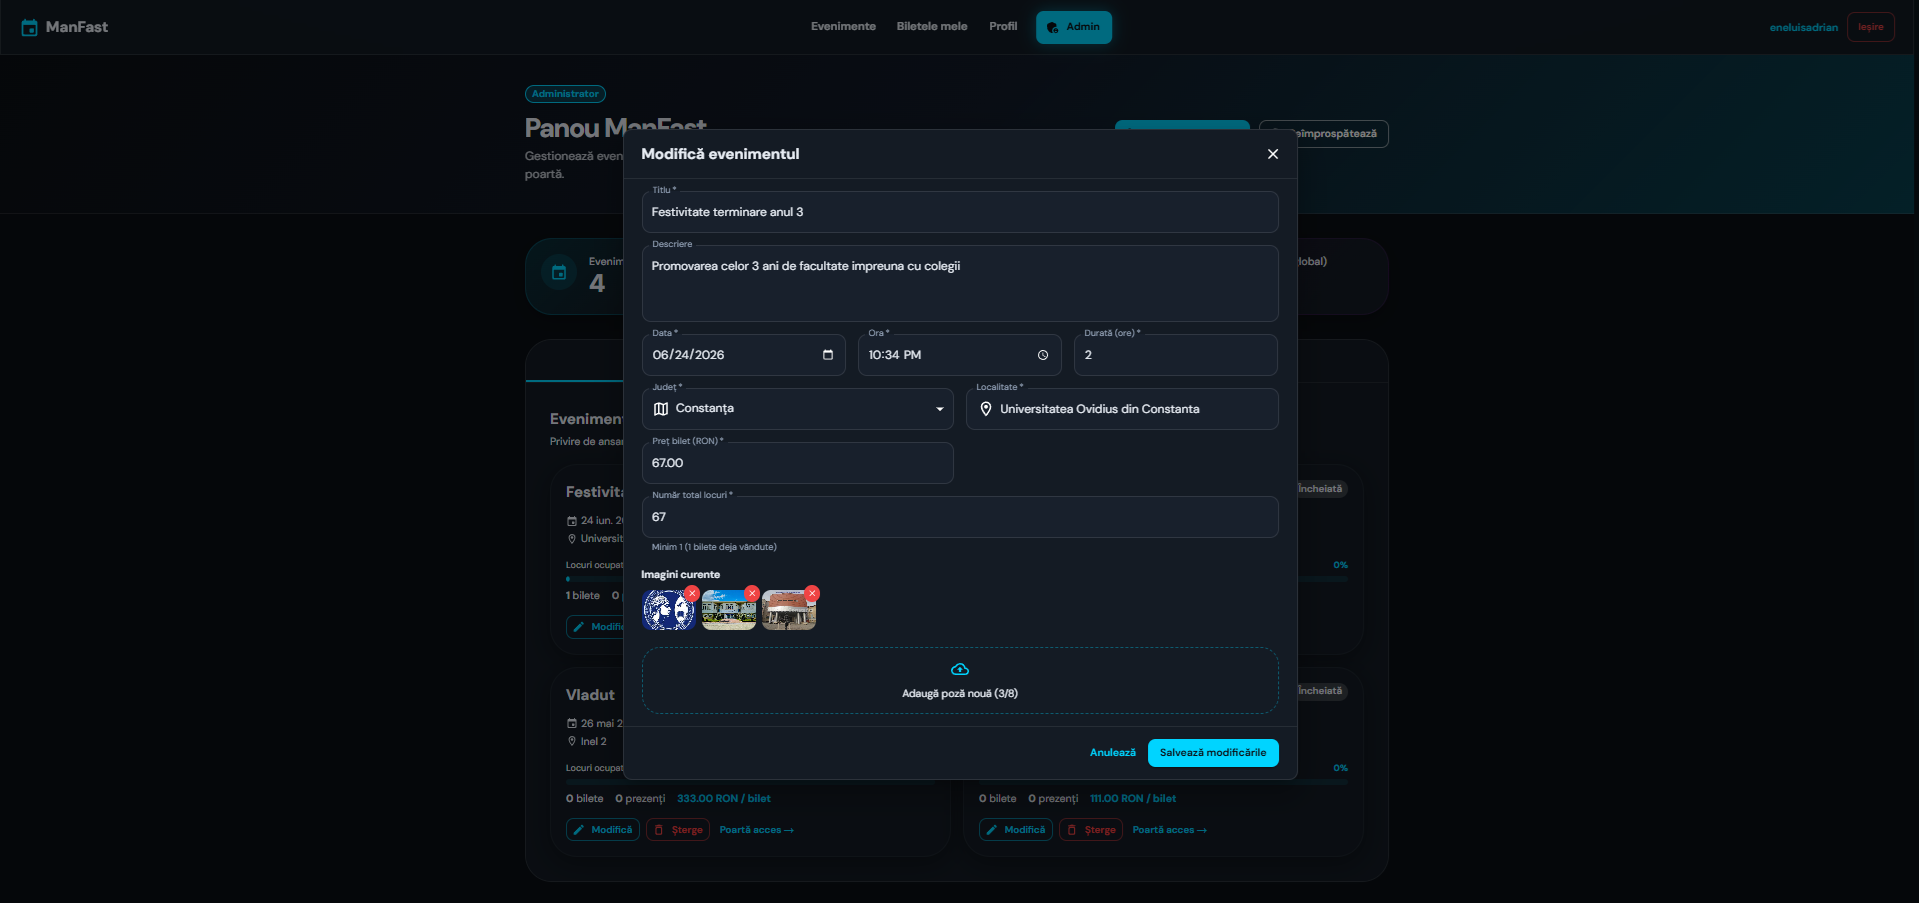
\includegraphics[width=1\textwidth]{Dialog editare eveniment.png}
	\caption{Dialog editare eveniment}
	\label{fig:l2f1}
\end{figure}

\subsection{Check-in participant}

Marcarea unui participant ca prezent (buton check-in sau toggle)

\begin{figure}[htbp]
	\centering
	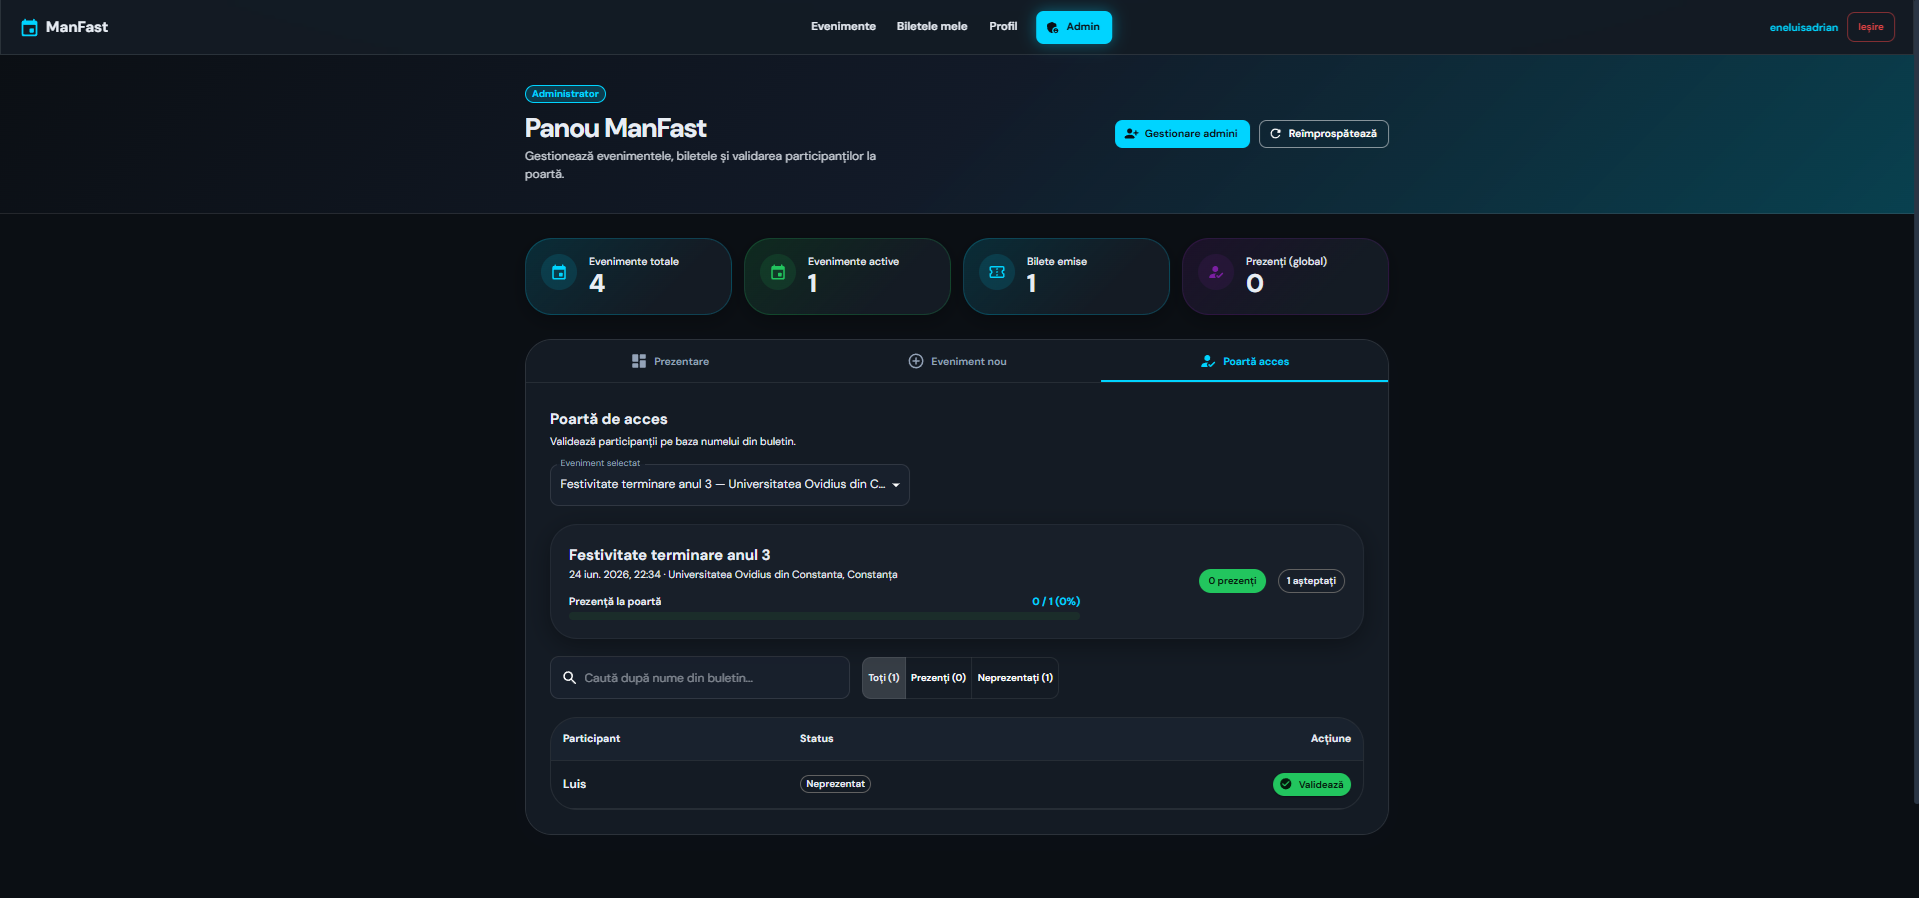
\includegraphics[width=1\textwidth]{Check-in participant.png}
	\caption{Check-in participant}
	\label{fig:l2f1}
\end{figure}

\begin{figure}[htbp]
	\centering
	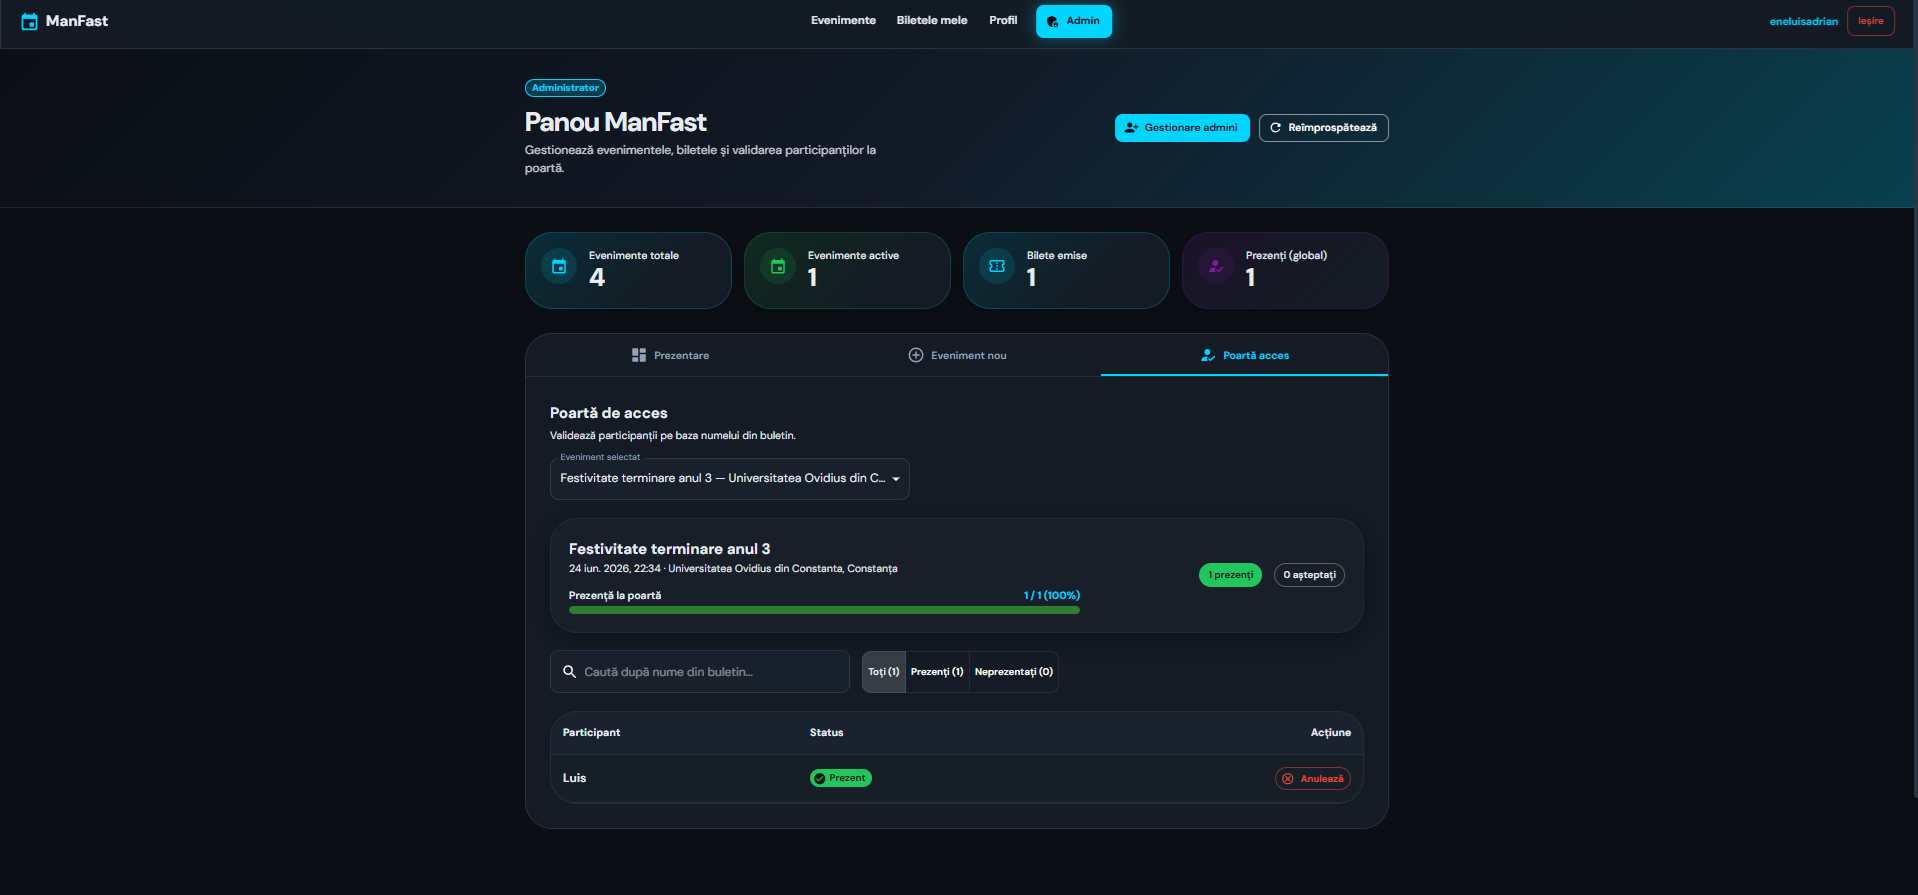
\includegraphics[width=1\textwidth]{Check-in participant2.png}
	\caption{Check-in participant validat}
	\label{fig:l2f1}
\end{figure}

\subsection{Gestionare administratori}

Dialog promovare sau revocare admin cu parol\u a autorizare.

\begin{figure}[htbp]
	\centering
	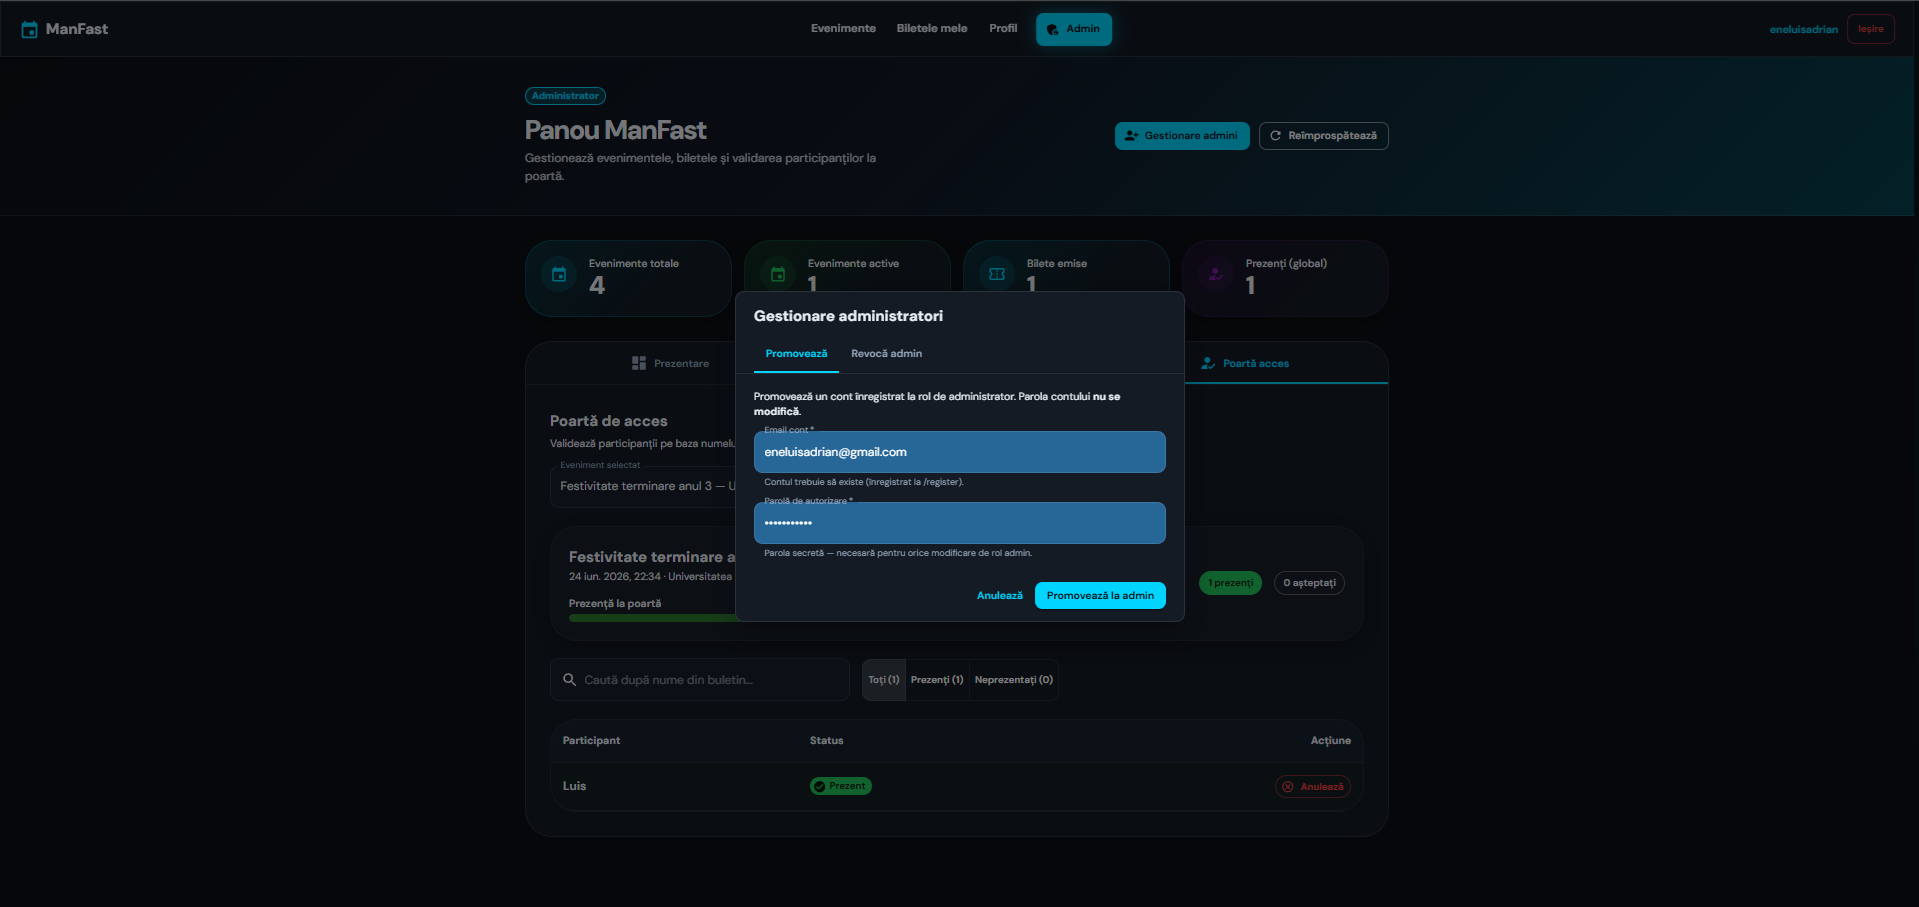
\includegraphics[width=1\textwidth]{Gestionare administratori.png}
	\caption{ Gestionare administratori}
	\label{fig:l2f1}
\end{figure}

\subsection{Conferin\c t\u a sau simpozion}

Pagina de detalii poate include \^in descriere: programul pe zile, lista speakerilor, link-uri c\u atre site-ul conferin\c tei. Imaginile \^inc\u arcate pot fi logo-ul evenimentului \c si fotografii din edi\c tii anterioare. Filtrele de pe Home permit g\u asirea conferin\c telor dintr-un anumit jude\c t sau dat\u a — util pentru participan\c ti care caut\u a evenimente academice regionale.

Formularul de cump\u arare bilet colecteaz\u a numele participantului (pentru ecuson sau list\u a oficial\u a). Dup\u a plat\u a, ,,Biletele mele`` afi\c seaz\u a evenimentul ca ,,viitor`` p\^an\u a la data desf\u a\c sur\u arii; ulterior trece automat \^in ,,trecute``.

\subsection{Concert sau spectacol}

Organizatorul pune accent pe elementele vizuale: mai multe imagini (arti\c sti, poster), descriere atractiv\u a, pre\c t \c si locuri limitate pentru a crea urgen\c t\u a. Utilizatorii pot cump\u ara bilete pentru mai multe persoane introduc\^and c\^ate un nume per c\^amp — potrivit pentru ie\c sirile \^in grup.

Navbar-ul \c si tema dark ofer\u a un aspect modern, aliniat la a\c stept\u arile publicului t\^an\u ar pentru evenimente culturale. Pagina de succes dup\u a Stripe confirm\u a achizi\c tia \c si \linebreak redirec\c tioneaz\u a spre bilete.

\subsection{Meeting, workshop sau seminar}

Pentru evenimente profesionale cu num\u ar mic de locuri, administratorul poate urm\u ari \^in timp real c\^ate locuri au r\u amas disponibile. Check-in-ul la intrare \^in sala de training confirm\u a prezen\c ta pentru certificat sau raport HR. Resetarea parolei \c si editarea profilului permit participan\c tilor s\u a-\c si men\c tin\u a contul pe termen lung, pentru evenimente recurente organizate de aceea\c si entitate.

\subsection{Eveniment sportiv (caz secundar)}

La competi\c tii, numele de pe bilet poate corespunde actului de identitate al sportivului. Admin-ul bifeaz\u a check-in la \^inregistrarea la concurs. Interfa\c ta nu afi\c seaz\u a distinc\c tii specifice (categorie greutate, gen), dar fluxul tehnic este identic — organizatorul completeaz\u a manual detaliile \^in titlu \c si descriere.

\subsection{Recomand\u ari pentru capturi de ecran (capitol 4)}

Pentru o documenta\c tie reprezentativ\u a, autorul poate crea \^in baza de date trei evenimente demonstrative:
\begin{itemize}
	\item ,,Conferin\c ta Na\c tional\u a Informatic\u a 2026`` — accent pe descriere lung\u a \c si dat\u a.
	\item ,,Concert Jazz Constan\c ta`` — accent pe galerie imagini.
	\item ,,Workshop React pentru \^Incep\u atori`` — accent pe locuri limitate (ex. 25).
\end{itemize}

Capturile din figurile 4.1--4.8 pot folosi oricare dintre aceste evenimente; important este ca textul lucr\u arii s\u a reflecte diversitatea cazurilor, nu doar un singur domeniu.


\subsection{Accesibilitate \c si public larg}

Indiferent de categorie, formularele respect\u a etichetare clar\u a, mesaje de eroare \^in rom\^an\u a \c si layout responsive. Participan\c tii mai pu\c tin obi\c snui\c ti cu tehnologia (ex. invita\c ti la conferin\c t\u a) beneficiaz\u a de flux liniar: Home $\rightarrow$ Detalii $\rightarrow$ Login/Register $\rightarrow$ Plat\u a $\rightarrow$ Bilete.

Aceste exemple completeaz\u a descrierea interfe\c tei \c si leag\u a capturile de ecran de cazuri reale de utilizare \^in domeniul conferin\c telor, concertelor \c si meeting-urilor.